\documentclass[tikz,border=10pt]{standalone}
\usepackage{amsmath,amssymb}
\usepackage{newpxtext,newpxmath}
\usepackage{pgfplots}
\pgfplotsset{compat=1.18}
\usetikzlibrary{arrows.meta}

\definecolor{inkDark}{HTML}{1E293B}
\definecolor{slateSub}{HTML}{334155}
\definecolor{pathBlue}{HTML}{005A9C}
\definecolor{accentRed}{HTML}{B91C1C}
\definecolor{accentTeal}{HTML}{0E6251}
\definecolor{accentAmber}{HTML}{B45309}
\definecolor{bandBlue}{HTML}{DBEAFE}
\definecolor{boxFill}{HTML}{F8FAFC}

\begin{document}
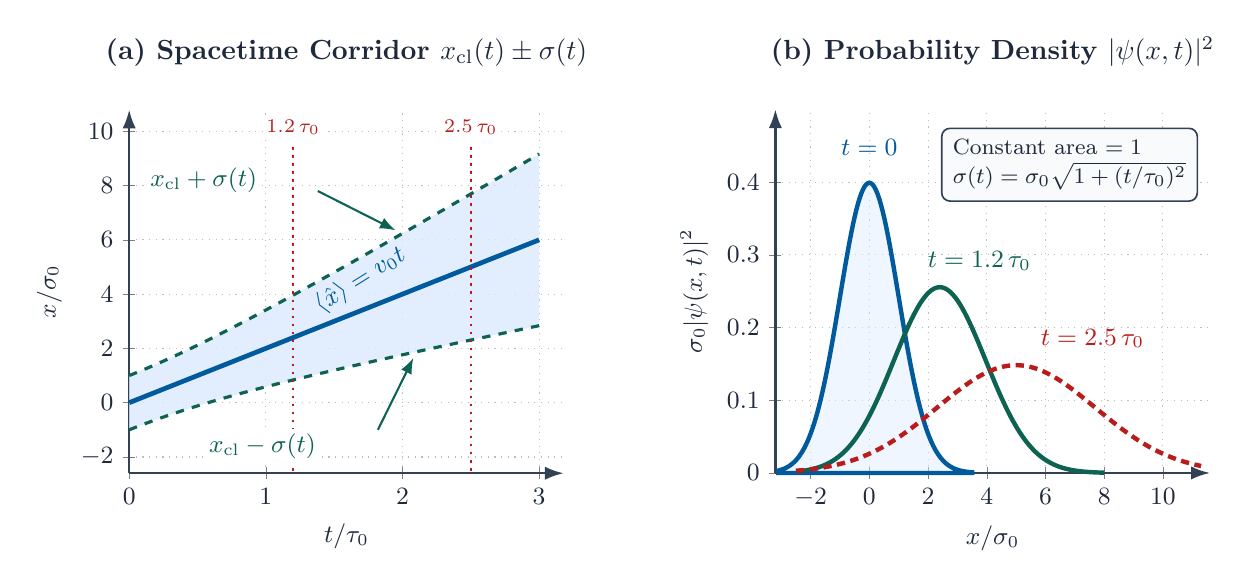
\begin{tikzpicture}[every node/.style={text=inkDark}]

    % =========================================================
    % Panel (a): Spacetime corridor of a spreading wave packet
    % Units: sigma_0 = 1, tau_0 = 2 m sigma_0^2 / hbar = 1, v_0 = 2
    % =========================================================
    \begin{axis}[
        name=axA,
        width=7.1cm,
        height=6.2cm,
        title={(a) Spacetime Corridor $x_{\mathrm{cl}}(t) \pm \sigma(t)$},
        title style={font=\bfseries\normalsize, text=inkDark, yshift=6pt},
        xmin=0, xmax=3.18,
        ymin=-2.6, ymax=10.8,
        axis lines=left,
        axis line style={-{Latex[length=2.4mm,width=1.7mm]}, line width=0.9pt, draw=slateSub},
        xlabel={$t / \tau_0$},
        ylabel={$x / \sigma_0$},
        xlabel style={font=\small, text=inkDark},
        ylabel style={font=\small, text=inkDark},
        xtick={0, 1, 2, 3},
        ytick={-2, 0, 2, 4, 6, 8, 10},
        tick label style={font=\small, text=inkDark},
        grid=major,
        grid style={dotted, slateSub, opacity=0.35},
        clip=false
    ]
        % Fill +-1 sigma corridor using exact closed path
        \addplot[draw=none, fill=bandBlue, opacity=0.80]
            coordinates {
                (0.0, 1.000) (0.3, 1.644) (0.6, 2.366) (0.9, 3.145) (1.2, 3.962)
                (1.5, 4.803) (1.8, 5.659) (2.1, 6.526) (2.4, 7.400) (2.7, 8.279) (3.0, 9.162)
                (3.0, 2.838) (2.7, 2.521) (2.4, 2.200) (2.1, 1.874) (1.8, 1.541)
                (1.5, 1.197) (1.2, 0.838) (0.9, 0.455) (0.6, 0.034) (0.3, -0.444) (0.0, -1.000)
            } -- cycle;

        % +-1 sigma boundaries
        \addplot[domain=0:3.0, samples=80, line width=1.15pt, draw=accentTeal, dashed]
            {2*x + sqrt(1 + x*x)};
        \addplot[domain=0:3.0, samples=80, line width=1.15pt, draw=accentTeal, dashed]
            {2*x - sqrt(1 + x*x)};

        % Classical trajectory x_cl(t) = v_0 t
        \addplot[domain=0:3.0, samples=50, line width=1.7pt, draw=pathBlue]
            {2*x};

        % Slice markers at t = 1.2 and 2.5 with clean top labels
        \draw[dotted, line width=0.9pt, draw=accentRed] (axis cs:1.2, -2.5) -- (axis cs:1.2, 9.6);
        \draw[dotted, line width=0.9pt, draw=accentRed] (axis cs:2.5, -2.5) -- (axis cs:2.5, 9.6);
        \node[font=\scriptsize\bfseries, text=accentRed, fill=white, inner sep=1pt] at (axis cs:1.2, 10.15) {$1.2\,\tau_0$};
        \node[font=\scriptsize\bfseries, text=accentRed, fill=white, inner sep=1pt] at (axis cs:2.5, 10.15) {$2.5\,\tau_0$};

        % Labels cleanly offset from curves & dotted lines
        \node[font=\small\bfseries, text=pathBlue, rotate=32, above=2pt] at (axis cs:1.80, 3.65) {$\langle \hat x\rangle = v_0 t$};

        \node[font=\small, text=accentTeal, fill=white, inner sep=1.5pt, anchor=west] at (axis cs:0.12, 8.20) {$x_{\mathrm{cl}} + \sigma(t)$};
        \draw[-{Latex[length=2.0mm]}, draw=accentTeal, line width=0.75pt] (axis cs:1.38, 7.80) -- (axis cs:1.95, 6.35);

        \node[font=\small, text=accentTeal, fill=white, inner sep=1.5pt, anchor=west] at (axis cs:0.55, -1.60) {$x_{\mathrm{cl}} - \sigma(t)$};
        \draw[-{Latex[length=2.0mm]}, draw=accentTeal, line width=0.75pt] (axis cs:1.82, -1.00) -- (axis cs:2.08, 1.65);
    \end{axis}

    % =========================================================
    % Panel (b): Probability density profiles |psi(x,t)|^2
    % =========================================================
    \begin{axis}[
        name=axB,
        at={(axA.outer east)},
        anchor=outer west,
        xshift=0.95cm,
        width=7.1cm,
        height=6.2cm,
        title={(b) Probability Density $|\psi(x,t)|^2$},
        title style={font=\bfseries\normalsize, text=inkDark, yshift=6pt},
        xmin=-3.2, xmax=11.6,
        ymin=0, ymax=0.50,
        axis lines=left,
        axis line style={-{Latex[length=2.4mm,width=1.7mm]}, line width=0.9pt, draw=slateSub},
        xlabel={$x / \sigma_0$},
        ylabel={$\sigma_0 |\psi(x,t)|^2$},
        xlabel style={font=\small, text=inkDark},
        ylabel style={font=\small, text=inkDark},
        xtick={-2, 0, 2, 4, 6, 8, 10},
        ytick={0, 0.1, 0.2, 0.3, 0.4},
        tick label style={font=\small, text=inkDark},
        grid=major,
        grid style={dotted, slateSub, opacity=0.35},
        clip=false
    ]
        % t = 0: mu=0, sigma=1, peak = 0.3989
        \addplot[domain=-3.1:3.5, samples=120, line width=1.6pt, draw=pathBlue, fill=bandBlue, fill opacity=0.45]
            {0.39894 * exp(-0.5 * x*x)} \closedcycle;

        % t = 1.2: mu=2.4, sigma=sqrt(2.44)=1.562, peak = 0.2554
        \addplot[domain=-2.5:8.0, samples=140, line width=1.6pt, draw=accentTeal]
            {0.25540 * exp(-0.5 * ((x-2.4)/1.56205)^2)};

        % t = 2.5: mu=5.0, sigma=sqrt(7.25)=2.6926, peak = 0.14816
        \addplot[domain=-2.5:11.3, samples=160, line width=1.6pt, draw=accentRed, densely dashed]
            {0.14816 * exp(-0.5 * ((x-5.0)/2.69258)^2)};

        % Direct curve labels near peaks
        \node[font=\small\bfseries, text=pathBlue] at (axis cs:0.0, 0.448) {$t = 0$};
        \node[font=\small\bfseries, text=accentTeal] at (axis cs:3.75, 0.292) {$t = 1.2\,\tau_0$};
        \node[font=\small\bfseries, text=accentRed] at (axis cs:7.60, 0.185) {$t = 2.5\,\tau_0$};

        % Annotation box cleanly inside plot bounds
        \node[
            draw=slateSub, line width=0.6pt, rounded corners=3pt,
            fill=boxFill, inner sep=4pt, font=\footnotesize, text=inkDark, align=left,
            anchor=north east
        ] at (axis cs:11.2, 0.475) {Constant area $= 1$\\[1pt] $\sigma(t) = \sigma_0\sqrt{1+(t/\tau_0)^2}$};
    \end{axis}

\end{tikzpicture}
\end{document}
